\documentclass{article}
\usepackage[utf8]{inputenc}
\usepackage{url,amsmath,graphicx,amssymb,booktabs}
\usepackage[top=1.5cm, bottom=1.5cm, left=2.5cm, right=2.5cm]{geometry}
\usepackage{tikz}
\usetikzlibrary{positioning,shapes.multipart}

\newtheorem{theorem}{Theorem}
\newtheorem{lemma}{Lemma}
\newtheorem{corollary}{Corollary}
\newtheorem{definition}{Definition}
\newtheorem{Proposition}{Proposition}

\newcommand{\Prob}{\mathbb{P}}
\newcommand{\E}{\mathbb{E}}
\newcommand{\Space}{\mathbb{S}}
\newcommand{\Var}{\text{Var}}
\newcommand{\MR}{\mathcal{R}}
\newcommand{\MT}{\mathcal{T}}

\title{MA3676 - Stochastic Models}
\author{1720996}
\date{\today}

\begin{document}

\maketitle

\tableofcontents

\section{Week 1}
\subsection{Axioms of Probability and conditional probabilities}
\subsubsection{Axioms of probability}
\begin{itemize}
    \item \textbf{Axiom $1$}: To each event $E$ there corresponds a number $\Prob[E]\geq0$, where $\Prob[E]$ is called the probability of $E$.
    \item \textbf{Axiom $2$}: $\Prob[\Space]=1$.
    \item \textbf{Axiom 3}: If events $A_1,\,A_2,\,A_3,\ldots$ are mutually exclusive then
    \begin{equation}
        \Prob\left[ \bigcup_{i=1}^\infty A_i \right] = \sum_{i=1}^\infty \Prob[A_i].
    \end{equation}
\end{itemize}

\subsubsection{Conditional probability}
\begin{definition}
\begin{equation}
    \Prob[A\vert B]=\frac{\Prob[A\cap B]}{\Prob[B]}.
\end{equation}
\end{definition}

\begin{definition}
    Two events $A$ and $B$ are independent if $\Prob[A\cap B]=\Prob[A]\Prob[B]$.
\end{definition}

\begin{definition}
    \begin{equation}
        \Prob[A_i\vert B] = \frac{\Prob[A_i]\Prob[B\vert A_i]}{\sum_{j+1}^n\Prob[A_j]\Prob[B\vert A_j]}.
    \end{equation}
\end{definition}

\section{Week 2}
\subsection{Discrete random variables}
\subsubsection{Bernoulli distribution}
\begin{definition}
    If the probability of event $E$ is $p$, then the variable $I_E$ is an indicator variable, which is said to follow the Bernoulli distribution with parameter $P$
    \begin{equation}
        \Prob[I_E=1]=p,\,\Prob[I_E=0]=1-p,
    \end{equation}
    or in shorthand, $\Prob[1]=p,\,\Prob[0]=1-p$.
\end{definition}

\subsubsection{Independence of random variables}
\begin{definition}
    Two random variables $X$ and $Y$ are independent if for any possible value $x$ of $X$ and any possible value $y$ of $Y$ the events $\{X=x\}$ and $\{Y=y\}$ are independent.
\end{definition}

\subsubsection{Binomial distribution}
\begin{definition}
    \begin{equation}
        \Prob[\{ Y_n=m \}] = \begin{pmatrix} n \\ m \end{pmatrix}p^m1^{n-m}.
    \end{equation}
\end{definition}

\subsubsection{Poisson distribution}
\begin{definition}
    \begin{equation}
        P(m) = \frac{\lambda^m}{m!}e^{-\lambda}.
    \end{equation}
\end{definition}

\subsubsection{Geometric Distribution}
\begin{definition}
    \begin{equation}
        P(n) = p^{n-1}(1-p).
    \end{equation}
\end{definition}


\subsection{Sums and Series}
\subsubsection{Finite geometric sum}
\begin{definition}
    \begin{equation}
        S_n=\sum_{k=0}^n a^k= 1+a+a^2+\cdots+a^n,
    \end{equation}
    hence
    \begin{equation}
        S_n = \frac{1-a^{n+1}}{1-a}.
    \end{equation}
\end{definition}
\subsubsection{Convergence of series}
In order for the series $\sum_{n=1}^\infty b_n$ to converge, the limit $\lim_{A\to\infty}(b_1+b_2+b_3+\cdots+b_A)$ must exist. \\
A necessary condition for the convergence of this series is that the limit of the sequence $b_n$ exists and is equal to $0$:
\begin{equation}
    \lim_{n\to\infty} b_n=0
\end{equation}

\subsubsection{Series examples}
\begin{definition}
Geometric series:
    \begin{equation}
        \sum_{n=0}^\infty a^n = \frac{1}{1-a}.
    \end{equation}
\end{definition}
\begin{definition}
Power series:
    \begin{equation}
        \sum_{n=0}^\infty \frac{x^n}{n!}=e^x.
    \end{equation}    
\end{definition}
\begin{definition}
    Logarithmic series:
    \begin{equation}
        \sum_{n=1}^\infty \frac{x^n}{n} = -ln(1-x).
    \end{equation}
\end{definition}
\begin{definition}
    Trigonometric series:
    \begin{equation}
        \sum_{n=0}^\infty \frac{(-1)^n x^{2n+1}}{(2n+1)!} = \sin x,
    \end{equation}
    \begin{equation}
        \sum_{n=0}^\infty \frac{(-1)^n x^{2n}}{(2n)!} = \cos x.
    \end{equation}
\end{definition}

\section{Week 3}
\subsection{Expectation value}
\subsubsection{Expectation of a random variable}
\begin{definition}
    Consider a discrete random variable $X$ which takes its values in a set $\{ x_1,\,x_2,\,\ldots \}$ with probabilities $\Prob[\{X=x_i\}]=p_i$. Then, the expectation value of $X$ is defined as
    \begin{equation}
        \E[X] = \sum_i x_i p_i.
    \end{equation}
\end{definition}
\subsubsection{Expectation of functions of random variables}
\begin{definition}
    \begin{equation}
        \E[g(X)] = \sum_i g(x_i)p_i.
    \end{equation}
\end{definition}
\subsubsection{Linearity of expectation}
\begin{definition}
    \begin{equation}
        \E[aX+bY] = a\E[X]+b\E[Y].
    \end{equation}
\end{definition}


\subsection{Expectation and variance values}
\subsubsection{Variance of a random variable}
\begin{definition}
    \begin{equation}
        \Var[X] =\E[(X-\E[X])^2]. 
    \end{equation}
\end{definition}

\subsubsection{Variance of a binomial random variable}
\begin{definition}
    \begin{equation}
        \Var[\sum_{i+1}^n X_i] = n\Var[X].
    \end{equation}
\end{definition}

\section{Week 4}
\subsection{Generating functions}
\subsubsection{The concept of a stochastic process: terminology}
\begin{itemize}
    \item The collection of all indices marking the random variables: the index set.
    \item All possible values of each $X_i$: the state space.
    \item Particular values $x_i$ taken by $X_i$ are the states of the process.
    \item The elements of the index set are conventionally called times.
    \item The whole collection of values $\{ x_i \}_{i=1}^N$ is a realisation of the process run for $N$ steps.
    \item A stochastic process can be viewed as a single, multi-component random variable.
\end{itemize}

\subsubsection{Definitions and basic properties}
\begin{definition}
    A (discrete) ``Random Walk'' is a stochastic process $S_n$ which can be represented as a sum of random variables (``steps''):
    \begin{equation}
        S_n = S_0+\sum_{k=1}^n X_k.
    \end{equation}
\end{definition}
\begin{definition}
    A ``Simple Random Walk'' is obtained if $X_k$ are independently identically distributed (i.i.d.) modified Bernoulli random variables taking values in the set $\{-1,\,1\}$, i.e.
    \begin{equation}
        \Prob[X_k=1]=p,\quad\Prob[X_k=-1]=1,\quad p+q=1,\quad \forall k\in \mathbb{N}. \nonumber
    \end{equation}
\end{definition}
\subsubsection{Generating functions: definition}
\begin{definition}
    Consider a discrete random variable $X$, and denote $\Prob[X=n]=p_n$. We now define the corresponding generating function $G(s)$ as
    \begin{equation}
        G(s) = \E[s^X].
    \end{equation}
\end{definition}
\begin{definition}
    \begin{equation}
        G(s) = \sum_n p_n s^n.
    \end{equation}
\end{definition}
\subsubsection{Expectation of a generating function}
\begin{definition}
    \begin{equation}
        \E[X]=G^\prime (1)
    \end{equation}
\end{definition}
\subsubsection{Variance of a generating function}
\begin{definition}
    \begin{equation}
        \Var[X] = G^{\prime\prime}(1) + G^\prime(1)-G^\prime(1)^2
    \end{equation}
\end{definition}



\section{Week 5}
\subsection{Random Walks}
\subsubsection{Probability mass function}
\begin{definition}
    \begin{equation}
        G_{S_n}=\sum_{m=0}^n \begin{pmatrix} n \\ m \end{pmatrix} p^{n-m}q^{m}s^{n-2m},
    \end{equation}
\end{definition}
where the powers of $s$ correspond to values of $S_n$.
\begin{definition}
    The probability of displacement by $k$ is denoted as
    \begin{equation}
        P_k^{(n)} \equiv \Prob[S_n-S_0=k]=\begin{pmatrix} n \\ \frac{n-k}{2} \end{pmatrix}p^{\frac{n+k}{2}}q^{\frac{n-k}{2}}.
    \end{equation}
\end{definition}
\subsubsection{General random walks}
\begin{theorem}
    Suppose $S_n = \sum_{k=1}^n X_k$ is a random walk such that $X_k$'s are i.i.d. random variables, characterised by a generating function $G_X(s)=\E[s^X]$. Then, the generating function of $S_n$ is
    \begin{equation}
        G_{S_n}(s)=G_X(s)^n
    \end{equation}
\end{theorem}
\subsubsection{Returning to the initial position}
\begin{theorem}
    For an unrestricted unbiased one-dimensional random walk the probability of return $\MR=1$.
\end{theorem}
Here, the number of returns $N$ to the state $i$ is represented by $\E[N]$.
\begin{lemma}
    \begin{equation}
        E[N]=\sum_{n=1}^\infty P_0^{(n)}.
    \end{equation}
\end{lemma}
\begin{lemma}
    If $\MR<1$, then
    \begin{equation}
        \E[N]=\frac{\MR}{1-\MR}.
    \end{equation}
\end{lemma}

\section{Week 6}
\subsection{Gambler's ruin}
Denote events such that:
\begin{itemize}
    \item $R_n$: player A is eventually ruined starting from initial capital $n$.
    \item $W_n$: player A wins the first game starting from initial capital $n$.
    \item $L_n=\overline{W}_n$: player A loses the first game starting from initial capital $n$.
\end{itemize}
\subsubsection{Probability of ruin}
\begin{definition}
The probability of ruin of a player from initial capital $n$ is
    \begin{equation}
        \Prob[R_n] = \Prob[R_n\vert W_n]\Prob[W_n] + \Prob[R_n\vert L_n]\Prob[L_n],
    \end{equation}
    which simplifies to
    \begin{equation}
        P_n = pP_{n+1} +qP_{n-1},
    \end{equation}
    where $\Prob[R_n\vert L_n]=P_{n-1}$, $\Prob[R_n\vert W_n]=P_{n+1}$, $\Prob[W_n]=p$ and $\Prob[L_n]=q=1-p$. 
\end{definition}
\begin{definition}
    The probability of ruin from initial capital $a$ with total pool $a+b$ is given by
    \begin{equation}
        P_a=\frac{1-(1/p)^b}{(p/q)^a-(1/p)^b},
    \end{equation}
    where $p\neq q$. If $p=q=1/2$, then
    \begin{equation}
        P_a = \frac{b}{a+b}.
    \end{equation}
\end{definition}

\section{Week 7}
\subsection{First step decomposition}
\subsubsection{Time to absorption}
\begin{definition}
    Let $T_n$ be the random variable equal to the number of steps, starting from $n$, which the random walker will make before reaching wither of the boundaries. Denote as
    \begin{equation}
        \MT = \E[T_n] \nonumber
    \end{equation}
    the expected number of steps until the walker reaches either of the boundaries.
\end{definition}
\begin{definition}
    \begin{align}
        \MT_n &= A+B(q/p)^n+\frac{n}{q-p},\quad &p\neq q, \\
        \MT_n &= A+Bn-n^2,\quad &q=p=1/2.
    \end{align}
\end{definition}

\section{Week 8}
\subsection{Boundary Conditions}
Use first step decomposition on the boundary conditions to solve for A and B. Use examples to understand.

\section{Week 9}
\subsection{Introduction to Markov chains}
\begin{definition}
    A stochastic process $S_n$ with discrete state space and discrete index set is a Markov chain if $\Prob[S_{n+1}=j\vert S_0=i_0,\,S_1=i_1,\ldots,\,S_n=i_n]=\Prob[S_{n+1}=j\vert S_n=i_n],\,\forall j,\, i_0,\, i_1,\ldots,\,i_n$ and $\forall n\in \mathbb{N}$.
\end{definition}
This says that the future ($S_{n+1}$) is conditionally independent of the past $(\{ S_i \}_{i+1}^{n-1})$, given the knowledge of the present $S_n$.
\subsection{Markov chains}
\subsubsection{Random walk on a circle}
\begin{definition}
    Treat $p_{ij}$ as elements of an $(n\times n)$-matrix and $\mathbf{p}_i (n)$ as elements of an $n$-component row vector $\underline{\pi}(n)$ where the matrix $\mathbf{p}$ provides the full description of transitions and $\underline{\pi}$ the current states of each position. The total probability decomposition is a product of these such that:
    \begin{equation}
        \underline{\pi}(n+1)=\underline{\pi}(n)\mathbf{p}.
    \end{equation}
\end{definition}
\subsubsection{Chapman-Kolmogorov equation}
\begin{theorem}
    \begin{equation}
        \underline{\pi}(n)=\underline{\pi}(0)\mathbf{p}^n.
    \end{equation}
\end{theorem}

\subsubsection{Multiplying stochastic matrices}
\begin{theorem}
    A product of two (or more, by induction) stochastic matrices is again a stochastic matrix.
\end{theorem}

\section{Week 10}
\subsection{Markov chains}
\subsubsection{Equilibrium distribution}
\begin{theorem}
    If such a distribution exists, then it means formally the existence of the limit
    \begin{equation}
        \lim_{n\to\infty}\underline{\pi}(n)=\underline{\pi},
    \end{equation}
    and therefore
    \begin{equation}
        \underline{\pi} = \underline{\pi}\mathbf{p}.
    \end{equation}
\end{theorem}
\subsubsection{Matrix analysis of Markov chains}
\begin{theorem}
    $\lambda=1$ is an eigenvalue of any stochastic matrix $\mathbf{p}$.
\end{theorem}



\section{Week 17}


\subsection{Markov chains}

\subsubsection{Revisiting a position}
In a random walk with only $\pm1$ steps allowed, even positions can be reached with an even number of steps and vice versa. Thus a position $i$ can be revisited only after an even number of steps:
\begin{equation}
    P_{ii}^{(2m)} = \frac{(2m)!}{(m!)^2}p^m q^m\quad\text{and}\quad P_{ii}^{(2m-1)}=0
\end{equation}
for any initial position.
\begin{definition}
    A state, return to which is only possible after $m,\,2m,\,3m,\ldots$ steps is called periodic if $m\geq2$. Any other state is called aperiodic.
\end{definition}
\begin{definition}
    If the probability of return to a given state is equal to one, such a state is called recurrent. If this probability is less than one, the state is called transient.
\end{definition}
Note that this definition refers to the eventual probability of return, after an arbitrary number of steps.

\subsubsection{Classification of states}
These concepts apply to general discrete stochastic processes; in Markov chain applications $P_{ij}^{(m)}$ is $(p^{(m)})_{ij}$.
\begin{definition}
    A state $i$ is said to communicate with a state $j$ if it is possible eventually to reach $j$ starting from $i$, i.i., if $P_{ij}^{(m)}>0$ for some $m$.
\end{definition}
\begin{definition}
    States $i$ and $j$ intercommunicate if, in addition, $\exists m^\prime:P_{ji}^{(m^\prime)}>0$.
\end{definition}
This property is denoted as $i \leftrightarrow j$, and it is transitive:
\begin{equation}
    \text{If }i\leftrightarrow j\text{ and }j\leftrightarrow k\text{, then }i\leftrightarrow k.
\end{equation}

\subsubsection{Recurrence time}
Starting from a state $i$ the probability that the chain will next visit the same state after $m$ steps can be formally expressed ass
\begin{equation}
    f_{ii}^{(m)} = \Prob[(X_{n+m}=i\cap(X_{n+k}\neq i\forall k:1\leq k\leq m-1)\vert X_n=i)].
\end{equation}
The sum
\begin{equation}
    R_i = \sum_{m=1}^\infty f_{ii}^{(m)}
\end{equation}
is the probability of return, so $R_i = 1$ for a recurrent state $i$. This means that $f_{ii}^{(m)}$ has the meaning of a discrete probability distribution of recurrence ``times'' $T_i:f_{ii}^{(m)} = \Prob[T_i = m]$.\\
Thus $\mu_i = \E[T_i] = \sum_{m=1}^\infty mf_{ii}^{(m)}$ is the expectation of the recurrence time - often known as the mean recurrence time for a state $i$.
\begin{definition}
    Depending on whether $\mu_i$ is finite or infinite, all recurrent states are classified as positive-recurrent, or null-recurrent, respectively.
\end{definition}
\begin{definition}
    A positive-recurrent aperiodic state is ergodic.
\end{definition}
Two more special types of states are:
\begin{itemize}
    \item \textbf{Ephemeral} states: those states $i$ for which $p_{ki}=1$, for any $k$, and
    \item \textbf{Absorbing} states: those states $i$ for which $p_{ii}=1$.
\end{itemize}

\subsubsection{States are ``contagious''}
\begin{theorem}
    Two intercommunicating states must be of the same type.
\end{theorem}
\begin{theorem}
    Let $i$ be a recurrent state which communicates with $j$; then $i$ and $j$ intercommunicate, and $j$ is also a recurrent state of the same type and period as $i$.
\end{theorem}
\begin{corollary}
    A pair of recurrent states of the same type either intercommunicate, or neither of them communicates with the other.
\end{corollary}
\begin{corollary}
    A recurrent state of one type cannot communicate with a recurrent state of another type, nor with a transient state.
\end{corollary}
Note, a transient state can communicate with other transient states, as well as with both types of recurrent states.

\subsubsection{Closed sets of states}
\begin{definition}
    A set $C$ of states is closed if no state in $C$ communicates with any state outside of $C$. A sufficient condition for this is
    \begin{equation}
        p_{ij} = 0 \forall i\in C \text{ and } \forall j\notin C.
    \end{equation}
\end{definition}
\begin{definition}
    A closed set $C$ of states is irreducible if every pair of states in $C$ intercommunicate.
\end{definition}
\begin{itemize}
    \item Since a recurrent state cannot communicate with a transient state, the set of all recurrent states is closed, but not necessarily irreducible.
    \item If a closed set contains only one state then that state is absorbing.
    \item An irreducible closed set contains no smaller closed set.
\end{itemize}

\begin{theorem}
    The state space $\mathbb{S}$ of a Markov chain can be uniquely partitioned as
    \begin{equation}
        \mathbb{S} = T\cup C_1\cup C_2\cup\ldots \nonumber
    \end{equation}
    where $T$ is the set of all transient states, and $C_1,\,C_2,\ldots$ are irreducible closed sets of recurrent states, each set containing states of the same type. 
\end{theorem}
\begin{theorem}
    If the state space is finite, then at least one state is recurrent, and, assuming the chain is time-homogeneous, all recurrent states are positive recurrent.
\end{theorem}

\subsubsection{Corollaries of the decomposition theorem}
\begin{corollary}
    If the chain starts in, or eventually reaches one of the irreducible closed sets $C_r$, then it never leaves it. $C_r$ thus becomes the state space for the subsequent part of the realisation of the chain, and every state in $C_r$ is visited infinitely often. Thus the subset $C_r$, together with the corresponding transition probabilities, forms a Markov chain in it's own right.
\end{corollary}
\begin{corollary}
    If the chain starts in the set $T$ of transient states, then it either moves between states within $T$ forever, visiting any one state only a finite number of times, or it eventually enters one of the closed sets $C_r$ of recurrent states, and it remains in $C_r$ forever after.
\end{corollary}
\begin{figure}[ht]
    \begin{center}
        \resizebox{\textwidth}{!}{
            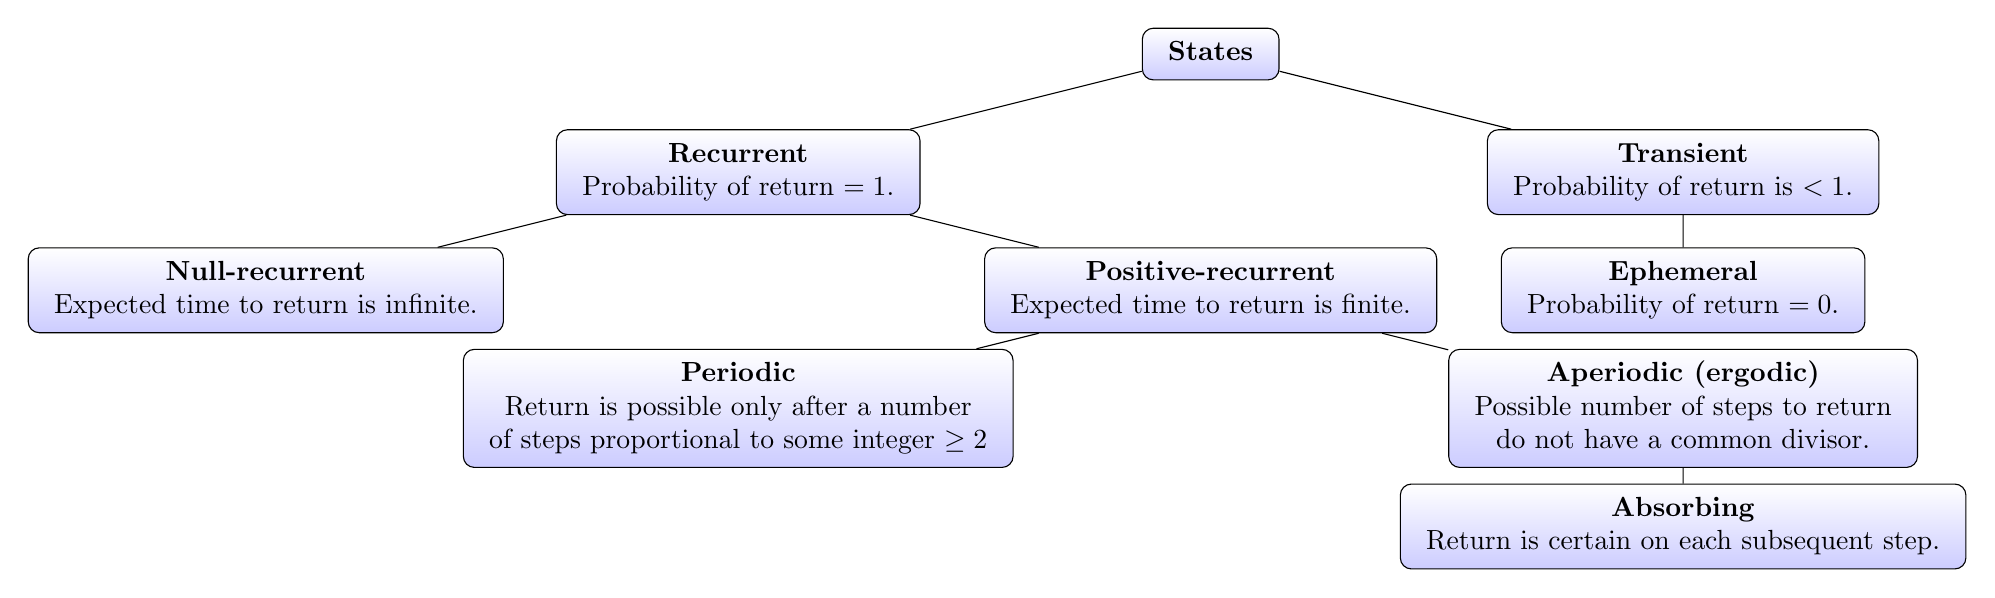
\begin{tikzpicture}[auto, sibling distance=120mm, text centered, 
              every node/.style = {shape=rectangle, rounded corners,
                draw,
                top color=white, bottom color=blue!20,}]]
              \node {\begin{tabular}{c} \textbf{States}\end{tabular}}
                child { node {\begin{tabular}{c} \textbf{Recurrent} \\ Probability of return $=1$. \end{tabular}}
                        child { node {\begin{tabular}{c}\textbf{Null-recurrent} \\ Expected time to return is infinite. \end{tabular}} }
                        child { node {\begin{tabular}{c} \textbf{Positive-recurrent} \\ Expected time to return is finite. \end{tabular}}
                            child { node {\begin{tabular}{c} \textbf{Periodic} \\ Return is possible only after a number \\ of steps proportional to some integer $\geq 2$ \end{tabular}} } 
                            child { node {\begin{tabular}{c} \textbf{Aperiodic (ergodic)} \\ Possible number of steps to return \\ do not have a common divisor. \end{tabular}} 
                                child { node {\begin{tabular}{c} \textbf{Absorbing} \\ Return is certain on each subsequent step. \end{tabular}} } } } } 
                child { node {\begin{tabular}{c} \textbf{Transient} \\ Probability of return is $<1$. \end{tabular}}
                    child { node {\begin{tabular}{c} \textbf{Ephemeral} \\ Probability of return $=0$. \end{tabular}} } };
            \end{tikzpicture}
        }
    \end{center}
\end{figure}

\subsubsection{Block matrices}
\begin{equation}
    M = \left(\begin{array}{c c c|c c|c c}
        1 & 2 & 3 & 4 & 5 & 6 & 7 \\
        8 & 9 & 10 & 11 & 12 & 13 & 14 \\
        \hline
        15 & 16 & 17 & 18 & 19 & 20 & 21 \\
        22 & 23 & 24 & 25 & 26 & 27 & 28 \\
        29 & 30 & 31 & 32 & 33 & 34 & 35
    \end{array}\right)
    =
    \left(\begin{array}{c c c}
        A & B & C \\
        D & E & F
    \end{array}\right). \nonumber
\end{equation}
Each of the blocks is defined in the obvious way:
\begin{equation}
    A =
    \begin{pmatrix}
        1 & 2 & 3 \\ 8 & 9 & 10
    \end{pmatrix},\quad
    B =
    \begin{pmatrix}
        4 & 5 \\ 11 & 12
    \end{pmatrix}\quad\text{etc.} \nonumber
\end{equation}
If we were to then have a matrix $N$ such that 
\begin{equation}
    N = 
    \begin{pmatrix}
        G & H \\ J & K \\ L & S
    \end{pmatrix} \nonumber
\end{equation}
that is the correct size so $MN$ exists, then
\begin{equation}
    MN = 
    \begin{pmatrix}
        A & B & C \\ D & E & F
    \end{pmatrix}
    \begin{pmatrix}
        G & H \\ J & K \\ L & S
    \end{pmatrix}
    =
    \begin{pmatrix}
        AG + BJ + CL & AH + BK + CS \\ DG + EJ + FL & DH + EK + FS
    \end{pmatrix}.
\end{equation}

\subsubsection{Permutations of rows and columns}
Consider a $3\times 3$-transition matrix, corresponding to states $1,\,2$ and $3$:
\begin{equation}
    \mathbf{p} =
    \begin{pmatrix}
        .1 & .7 & .2 \\ .3 & .5 & .2 \\ .2 & .4 & .4
    \end{pmatrix}. \nonumber
\end{equation}
If we now decide to list the states in the order $3,\,2,\,1$, then we need to swap the first and third row, \textbf{and} the first and third column, so that we get
\begin{equation}
    \begin{pmatrix}
        .4 & .4 & .2 \\ .2 & .5 & .3 \\ .2 & .7 & .1
    \end{pmatrix}. \nonumber
\end{equation}

\subsubsection{Reducibility}
\begin{theorem}
    If columns and rows of a square matrix $A$ can be permuted so that it acquires the form
    \begin{equation}
    A =
        \begin{pmatrix}
        B & 0 \\ C & D    
        \end{pmatrix}
    \end{equation}
    where $B$ (and hence $D$) are square matrices, and $0$ is a matrix consisting of all zeros, then $A$ is called reducible.
\end{theorem}
\begin{theorem}
    Transition matrix $\mathbf{p}$ of a decomposable (reducible) Markov chain is reducible.
\end{theorem}
Suppose $\Space = C\cup T$, with $k_C$ states in the closed set, and $k_T$ transient states. By definition of reducibility, the transition matrix $\mathbf{p}$ can be rearranged into the form
\begin{equation}
    \mathbf{p} = 
    \begin{pmatrix}
        P & 0 \\ R & Q    
        \end{pmatrix}.
\end{equation}
Here, $P$ corresponds to transitions among recurrent states of the closed set $C$, elements of $Q$ are probabilities of transitions among transient states, and elements of $R$ give the probabilities of transitions from transient to recurrent states. This form is retained after an arbitrary number of steps.

\section{Week 18}
\subsection{Markov Chains}
\subsubsection{Perron-Frobenius theorem}
\begin{definition}
    If all other eigenvalues $\lambda$ satisfy the strict inequality $\vert\lambda\vert<r$, then $A$ is called primitive.
\end{definition}
\begin{theorem}
    Suppose a matrix $A$ is irreducible, and all elements of $A$ are non-negative. Then the following statements are true:
    \begin{enumerate}
        \item $A$ has at least one real positive eigenvalue.
        \item The largest (if there is more than one) such real positive eigenvalue $r$ dominates all other eigenvalues: If $\alpha$ is any other eigenvalue of $A$, then $\vert\alpha\vert\leq r$.
        \item $r$ is non-degenerate, i.i., it is a simple root of the characteristic equations
        \begin{equation}
            \det(A_\lambda\mathbb{I})=0.
        \end{equation} \nonumber
        \item Corresponding to $r$ are the right and left eigenvectors all of whose components are positive. Conversely, the only eigenvectors whose components are positive are those corresponding to $r$.
        \item $r$ increases when any element of $A$ increases. Correspondingly, $r$ decreases when any element of $A$ decreases.
        \item If $A$ is not primitive, i.e., there are $d>1$ eigenvalues, such that $\vert\lambda\vert=r$, then they are all simple and different, and are located symmetrically on the unit circle in the complex plane: if they are numbered from $0$ to $d-1$, they can be written as
        \begin{equation}
            \lambda_k = re^{2\pi ik/d},
        \end{equation}
        with $k = 0,\,1,\ldots,\,d-1$. If there are two such roots, they are equal to $r$ and $-r$.\\
        Further, if $d>1$, the rows and columns of the matrix can be permuted to bring it to the block form
        \begin{equation}
            \begin{pmatrix}
                0 & A_1 & 0 & \cdots & 0 \\
                0 & 0 & A_2 & \cdots & 0 \\
                \vdots & \vdots & \vdots & \ddots & \vdots \\
                0 & 0 & 0 & \cdots & A_{d-1} \\
                A_d & 0 & 0 & \cdots & 0
            \end{pmatrix}. \nonumber
        \end{equation}
    \end{enumerate}
\end{theorem}

\subsubsection{Limiting behaviour}
\begin{corollary}
    If $A$ is irreducible and primitive, and $x$ and $y$ are the right (column) and left (row) eigenvectors of $A$ respectively, corresponding to the dominant eigenvalue $r$, and normalised so that $yx=1$, then
    \begin{equation}
        \lim_{n\to\infty}(1/r)^n A^n = x \otimes y,
    \end{equation}
    where $\otimes$ is used to denote the ``outer'' product of vectors: column times row.
\end{corollary}
Such products are known as dyadic products and the limits are uniform for all elements, so 
\begin{equation}
    \lim_{n\to\infty}(1/r)^n(A^n)_{ij} =x_i y_i. \nonumber
\end{equation}
\begin{theorem}
    For irreducible and primitive $\mathbf{p}$,
    \begin{equation}
        \lim_{n\to\infty}\mathbf{p}^n = e\otimes \pi. 
    \end{equation}
\end{theorem}
It follows that
\begin{corollary}
    If $\mathbf{p}$ is irreducible and primitive, there exists an equilibrium distribution.
\end{corollary}
LECTURE 22 SLIDE 13!


\section{Week 19}

\section{Week 20}

\section{Week 21}

\section{Week 23}

\end{document}
